\documentclass[a4paper,11pt]{article}
\usepackage{amsmath,amsthm,amsfonts,amssymb,amscd,amstext,vmargin,graphics,graphicx,tabularx,multicol} 
\usepackage[francais]{babel}
\usepackage[utf8]{inputenc}  
\usepackage[T1]{fontenc} 
\usepackage{pstricks-add,tikz,tkz-tab,variations}
\usepackage[autolanguage,np]{numprint} 

\setmarginsrb{1.5cm}{0.5cm}{1cm}{0.5cm}{0cm}{0cm}{0cm}{0cm} %Gauche, haut, droite, haut
\newcounter{numexo}
\newcommand{\exo}[1]{\stepcounter{numexo}\noindent{\bf Exercice~\thenumexo} : \marginpar{\hfill /#1}}
\reversemarginpar


\newcounter{enumtabi}
\newcounter{enumtaba}
\newcommand{\q}{\stepcounter{enumtabi} \theenumtabi.  }
\newcommand{\qa}{\stepcounter{enumtaba} (\alph{enumtaba}) }
\newcommand{\initq}{\setcounter{enumtabi}{0}}
\newcommand{\initqa}{\setcounter{enumtaba}{0}}

\newcommand{\be}{\begin{enumerate}}
\newcommand{\ee}{\end{enumerate}}
\newcommand{\bi}{\begin{itemize}}
\newcommand{\ei}{\end{itemize}}
\newcommand{\bp}{\begin{pspicture*}}
\newcommand{\ep}{\end{pspicture*}}
\newcommand{\bt}{\begin{tabular}}
\newcommand{\et}{\end{tabular}}
\renewcommand{\tabularxcolumn}[1]{>{\centering}m{#1}} %(colonne m{} centrée, au lieu de p par défault) 
\newcommand{\tnl}{\tabularnewline}

\newcommand{\bmul}[1]{\begin{multicols}{#1}}
\newcommand{\emul}{\end{multicols}}

\newcommand{\trait}{\noindent \rule{\linewidth}{0.2mm}}
\newcommand{\hs}[1]{\hspace{#1}}
\newcommand{\vs}[1]{\vspace{#1}}

\newcommand{\N}{\mathbb{N}}
\newcommand{\Z}{\mathbb{Z}}
\newcommand{\R}{\mathbb{R}}
\newcommand{\C}{\mathbb{C}}
\newcommand{\Dcal}{\mathcal{D}}
\newcommand{\Ccal}{\mathcal{C}}
\newcommand{\mc}{\mathcal}

\newcommand{\vect}[1]{\overrightarrow{#1}}
\newcommand{\ds}{\displaystyle}
\newcommand{\eq}{\quad \Leftrightarrow \quad}
\newcommand{\vecti}{\vec{\imath}}
\newcommand{\vectj}{\vec{\jmath}}
\newcommand{\Oij}{(O;\vec{\imath}, \vec{\jmath})}
\newcommand{\OIJ}{(O;I,J)}


\newcommand{\reponse}[1][1]{%
\multido{}{#1}{\makebox[\linewidth]{\rule[0pt]{0pt}{20pt}\dotfill}
}}

\newcommand{\titre}[5] 
% #1: titre #2: haut gauche #3: bas gauche #4: haut droite #5: bas droite
{
\noindent #2 \hfill #4 \\
#3 \hfill #5

\vspace{-1.6cm}

\begin{center}\rule{6cm}{0.5mm}\end{center}
\vspace{0.2cm}
\begin{center}{\large{\textbf{#1}}}\end{center}
\begin{center}\rule{6cm}{0.5mm}\end{center}
}



\begin{document}
\pagestyle{empty}
\titre{Contrôle : Les opérations et les périmètres }{Nom :}{Prénom :}{Classe}{Date}

\vspace*{0.25cm}
\begin{flushleft}
\begin{tabular}{|m{9.5cm}|m{1.25cm}|m{1.25cm}|m{1.25cm}|m{1.25cm}|m{1.25cm}|}
\hline 
\textbf{Compétences} & \begin{center}
\textbf{N.E.}
\end{center} & \begin{center}
\textbf{M.I.}
\end{center} & \begin{center}
\textbf{M.F.}
\end{center}  & \begin{center}
\textbf{M.S.}
\end{center} & \begin{center}
\textbf{T.B.M.}
\end{center} \\ 
\hline 
Je dois savoir prélever et organiser les informations nécessaires à la résolution de problèmes à partir de supports variés : textes, dessins, schémas, etc & & &  & &\\
\hline
Je dois savoir calculer avec des nombres décimaux, de manière exacte ou approchée, en utilisant des stratégies ou des techniques appropriées (mentalement, en ligne, ou en posant les opérations) & & &  & & \\ 
\hline 


\end{tabular}  
\end{flushleft}

\textit{N.E = Non évalué ; M.I. = Maîtrise insuffisante ; M.F. = Maîtrise fragile ; M.S. = Maîtrise satisfaisante ; T.B.M. = Très bonne maîtrise}\\

\vspace*{0.5cm}





Les exercices avec le signe  
\includegraphics[scale=0.3]{trefle.eps} sont à faire directement sur le sujet. Les autres se font sur la copie double.\\

\exo{5.5} 
\includegraphics[scale=0.3]{trefle.eps} Pour chacune des questions, entourer la bonne réponse :

\renewcommand\arraystretch{2}

\begin{flushleft}
\begin{tabular}{|c|m{10cm}|c|c|c|}
\hline 
 &  & \textbf{A} & \textbf{B} & \textbf{C} \\ 
\hline 
\textbf{1} & J'achète un pain à 1,75 euros, un croissant à 0,70 euros, un pain au chocolat à 0,90 euros et une brioche à 2,20 euros. Quel billet dois-je donner pour que la boulangère me rende le minimum de monnaie ?
 & 5 euros & 10 euros & 20 euros \\ 
\hline 
\textbf{2} & Un camion transporte 100 palettes.
Chaque palette contient 10 packs de 6 bouteilles d'eau minérale de 1,5 L.
Combien de litres d'eau transporte ce camion ?
 & 6 000 L & 117,5 L & 9 000 L \\ 
\hline 
\textbf{3} & Quelle masse obtient-on quand 
on ajoute 5 g à 2,3 hg ?
 & 2,8 hg	 & 2,35 hg	 & 2,305 hg \\ 
\hline 
\textbf{4} & Quel est le plus lourd : 8,7 kg ou 8 070 dg? & 
8,7 kg	 & 8 070 dg & 	C'est la même masse \\ 
\hline 
\textbf{5} & Le nombre 4 35$\star$ a un chiffre inconnu. Pourtant, on sait qu'il est multiple de 9. 
Donc le chiffre inconnu (remplacé par $\star$) peut être égal  à …
 & 6 & 1 & 3 \\ 
\hline 
\textbf{6} & Si le diviseur est 9, si le reste est 13  et si le quotient est 5  alors le dividende est … & 58		 & 74 & 122\\ 
\hline 
\end{tabular} 

\end{flushleft}

\vspace*{0.6cm}

\exo{3.5}\\
Paula fait des courses avec un billet de 20 euros en poche. Elle achète :\\
- 3 baguettes à 0,97 euro l'une, \\
- 2,7 kg de pommes à 1,50 euros le kg,\\
- 700 g de viande à 12,30 euros le kg.\\

$\rightarrow$  Combien lui reste-t-il après ses achats ? \textit{Faire apparaître les conversions éventuelles et vos calculs.}\\

\newpage


\exo{2.5}

\includegraphics[scale=0.7]{exodistance.eps} \\

\q Calculer les distances Rouen-St Malo et Amiens-Quimper.\\

\q Quelle distance cherche-t-on quand on propose le calcul suivant :   $610 - (411 +97)$ ?\\

\vspace*{0.5cm}





\vspace*{0.5cm}



\exo{2} 
\includegraphics[scale=0.3]{trefle.eps} En sachant que le côté d'un carreau mesure 1 cm. Déterminer le périmètre de chaque figure.

\bmul{2}

\includegraphics[scale=0.7]{carreauperimetre.eps} 

\columnbreak

\vspace*{1cm}

\bmul{2}

$P_{fig3}= . . . . .  . $\\

$P_{fig7}= . . . . .  . $\\

\columnbreak

$P_{fig4}= . . . . .  . $\\

$P_{fig8}= . . . . .  . $\\

\emul
\emul

\vspace*{0.5cm}


\exo{3} Calculs de périmètres\\

\initq 

\q Calculer le périmètre d'un rectangle de longueur 5 dm et de largeur 2,5 dm.\\

\q Calculer le périmètre d'un cercle de 50 cm de rayon.\\

\q Calculer la circonférence d'un cercle de diamètre 10 cm.\\

\vspace*{0.5cm}


\exo{4}



Les polygones ci-dessus ne sont pas représentés en grandeur réelle.\\
$\rightarrow$ \textbf{Calculer le périmètre de ces polygones.}\\

\qa \hspace*{6.5cm} \qa \\
 \includegraphics[scale=1]{exoperimetre.eps} \hspace*{1.75cm}  \includegraphics[scale=0.85]{exoperimetre3.eps} 


\vspace*{0.5cm}



\exo{} BONUS \\
 Benjamin possède des billes.\\	
 Il dit : « Je ne les ai pas comptées mais quand je les trie 5 par 5, il ne m'en reste pas. Quand je les trie 2 par 2, il m'en reste 1. Quand je les trie 6 par 6, il m'en reste 5. Je sais que j'en ai moins de 50 » .\\
 
Combien de billes Benjamin possède t-il ? Justifier votre réponse.\\

\end{document}
